\documentclass[12pt]{article}

%%%%%%%%%%%%%%%%%%%%%%%%%%%%%%%%%%%%%%%%%%%%%%%%%%%%%%%%%%%%%%%%%%%%%%%%%%%%%%%%%%%%%%%%%%%%%%%%%%%%
% Math
\usepackage{fancyhdr} 
\usepackage{amsfonts}
\usepackage{amsmath}
\usepackage{amssymb}
\usepackage{amsthm}
%\usepackage{dsfont}

%%%%%%%%%%%%%%%%%%%%%%%%%%%%%%%%%%%%%%%%%%%%%%%%%%%%%%%%%%%%%%%%%%%%%%%%%%%%%%%%%%%%%%%%%%%%%%%%%%%%
% Macros
\usepackage{calc}

%%%%%%%%%%%%%%%%%%%%%%%%%%%%%%%%%%%%%%%%%%%%%%%%%%%%%%%%%%%%%%%%%%%%%%%%%%%%%%%%%%%%%%%%%%%%%%%%%%%%
% Commands and Custom Variables	
\newcommand{\problem}[1]{\hspace{-4 ex} \large \textbf{Problem #1} }
\let\oldemptyset\emptyset
\let\emptyset\varnothing
\newcommand{\norm}[1]{\left\lVert#1\right\rVert}
\newcommand{\sint}{\text{s}\kern-5pt\int}
\newcommand{\powerset}{\mathcal{P}}
\renewenvironment{proof}{\hspace{-4 ex} \emph{Proof}:}{\qed}
\newcommand{\RR}{\mathbb{R}}
\newcommand{\NN}{\mathbb{N}}
\newcommand{\QQ}{\mathbb{Q}}
\newcommand{\ZZ}{\mathbb{Z}}
\newcommand{\CC}{\mathbb{C}}
\renewcommand{\Re}{\operatorname{Re}}
\renewcommand{\Im}{\operatorname{Im}}


%%%%%%%%%%%%%%%%%%%%%%%%%%%%%%%%%%%%%%%%%%%%%%%%%%%%%%%%%%%%%%%%%%%%%%%%%%%%%%%%%%%%%%%%%%%%%%%%%%%%
%page
\usepackage[margin=1in]{geometry}
\usepackage{setspace}
%\doublespacing
\allowdisplaybreaks
\pagestyle{fancy}
\fancyhf{}
\rhead{Shaw \space \thepage}
\setlength\parindent{0pt}

%%%%%%%%%%%%%%%%%%%%%%%%%%%%%%%%%%%%%%%%%%%%%%%%%%%%%%%%%%%%%%%%%%%%%%%%%%%%%%%%%%%%%%%%%%%%%%%%%%%%
%Code
\usepackage{listings}
\usepackage{courier}
\lstset{
	language=Python,
	showstringspaces=false,
	formfeed=newpage,
	tabsize=4,
	commentstyle=\itshape,
	basicstyle=\ttfamily,
}

%%%%%%%%%%%%%%%%%%%%%%%%%%%%%%%%%%%%%%%%%%%%%%%%%%%%%%%%%%%%%%%%%%%%%%%%%%%%%%%%%%%%%%%%%%%%%%%%%%%%
%Images
\usepackage{graphicx}
\graphicspath{ {images/} }
\usepackage{float}

%tikz
\usepackage[utf8]{inputenc}
\usepackage{pgfplots}
\usepgfplotslibrary{groupplots}

%%%%%%%%%%%%%%%%%%%%%%%%%%%%%%%%%%%%%%%%%%%%%%%%%%%%%%%%%%%%%%%%%%%%%%%%%%%%%%%%%%%%%%%%%%%%%%%%%%%%
%Hyperlinks
%\usepackage{hyperref}
%\hypersetup{
%	colorlinks=true,
%	linkcolor=blue,
%	filecolor=magenta,      
%	urlcolor=cyan,
%}

\begin{document}
	\thispagestyle{empty}
	
	\begin{flushright}
		Sage Shaw \\
		m565 - Fall 2017 \\
		\today
	\end{flushright}
	
{\large \textbf{HW 7}}\bigbreak

%%%%%%%%%%%%%%%%%%%%%%%%%%%%%%%%%%%%%%%%%%%%%%%%%%%%%%%%%%%%%%%%%%%%%%%%%%%%%%%%%%%%%%%%%%%%%%%%%%%%
\problem{1 (a)} The following code computes the error using the Trapezoidal rule applied to the functions
\begin{align*}
	I(f_1) & = \int_{-1}^1 (x-1)^2e^{-x^2}dx \\
	I(f_2) & = \int_{-1}^1 e^{\cos(\pi x)} dx
\end{align*}

\begin{lstlisting}
def trap_int(f, a, b, n):
	h = (b-a)/n
	x = a + h
	T = 0
	for i in range(n-1):
	T += f(x)
	x += h
	T += (f(a)+f(b))/2
	T *= h
	return T

def f1(x):
	return (x-1)**2 * np.exp(-x**2)

def f2(x):
	return np.exp( np.cos( np.pi*x ) )

int1_actual = 1.87259295726583875
int2_actual = 2.53213175550401667

def p1a():
	ns = [4, 8, 16, 32]
	T1 = []
	T2 = []
	for n in ns:
		T1.append( abs( trap_int(f1, -1, 1, n) - int1_actual ) )
		T2.append( abs( trap_int(f2, -1, 1, n) - int2_actual ) )
	latex_table( (ns, T1, T2), 
('$n$', '$I(f_1)$ error', '$I(f_2)$ error') )
\end{lstlisting}

	The output is displayed in the table below.
	\begin{center}
		\begin{tabular}{|c|c|c|}
			\hline
			$n$&$I(f_1)$ error&$I(f_2)$ error\\ \hline
			4&0.0312125372551&0.0109488793112\\ \hline
			8&0.0076967258198&3.98424961467e-07\\ \hline
			16&0.001918044355&4.4408920985e-16\\ \hline
			32&0.000479134582236&4.4408920985e-16\\ \hline
		\end{tabular}
	\end{center}

\bigbreak
%%%%%%%%%%%%%%%%%%%%%%%%%%%%%%%%%%%%%%%%%%%%%%%%%%%%%%%%%%%%%%%%%%%%%%%%%%%%%%%%%%%%%%%%%%%%%%%%%%%%
\problem{1 (b)} The following code does the same for the corrected Trapezoidal rule:

	\begin{lstlisting}
def df1(x):
	return 2*(x-1)*np.exp(-x**2) - 2*x*(x-1)**2 * np.exp(-x**2)

def df2(x):
	return -np.pi*np.sin(np.pi*x)*np.exp(np.cos(np.pi*x))

def trap_int_corrected(f, df, a, b, n):
	T = trap_int(f,a,b,n)
	h = (b-a)/n 
	return T - h**2/12*(df(b)-df(a))

def p1b():
	int1_actual = 1.87259295726583875
	int2_actual = 2.53213175550401667
	ns = [4, 8, 16, 32]
	T1 = []
	T2 = []
	for n in ns:
		T1.append( abs( trap_int_corrected(f1, df1, -1, 1, n)
- int1_actual ) )
		T2.append( abs( trap_int_corrected(f2, df2, -1, 1, n)
- int2_actual ) )
	latex_table( (ns, T1, T2), 
('$n$', '$I(f_1)$ error', '$I(f_2)$ error') ) 
	\end{lstlisting}
	
	\begin{center}
		\begin{tabular}{|c|c|c|}
			\hline
			$n$&$I(f_1)$ error&$I(f_2)$ error\\ \hline
			4&0.00055591715752&0.0109488793112\\ \hline
			8&3.25707953921e-05&3.98424961467e-07\\ \hline
			16&2.00559889851e-06&4.4408920985e-16\\ \hline
			32&1.24893210662e-07&4.4408920985e-16\\ \hline
		\end{tabular}
	\end{center}


\bigbreak
%%%%%%%%%%%%%%%%%%%%%%%%%%%%%%%%%%%%%%%%%%%%%%%%%%%%%%%%%%%%%%%%%%%%%%%%%%%%%%%%%%%%%%%%%%%%%%%%%%%%
\problem{1 (c)} To verify that the error of the Trapezoidal rule decreases like $\mathcal{O}(h^2)$ We plot $h^2$ with the error. (More data points have been calcluated for this plot.)
	\begin{figure}[H]
		\caption{Error of the trapezoidal rule}
		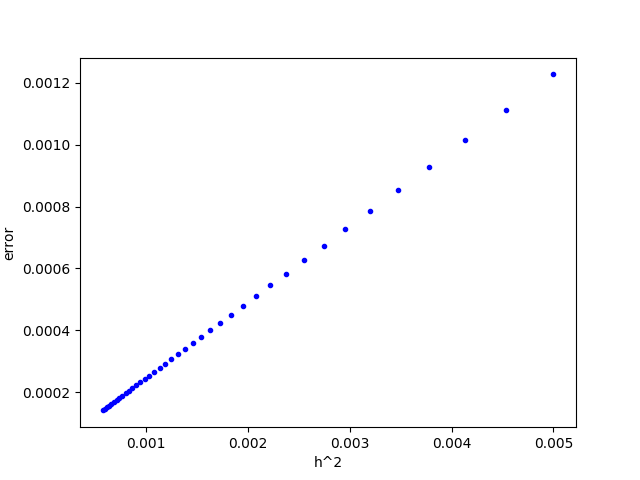
\includegraphics[width=.75\textwidth]{hw7_p1_fig1}
		\label{p1_T_err}
		\centering
	\end{figure}
	Since the plot is roughly linear we can confirm that the error decreases like $\mathcal{O}(h^2)$. \bigbreak

	Similarly a plot of $h^4$ with the error of the corrected Trapezoidal rule shows that its error decreaces according to $\mathcal{O}(h^4)$.
	\begin{figure}[H]
		\caption{Error of the corrected trapezoidal rule}
		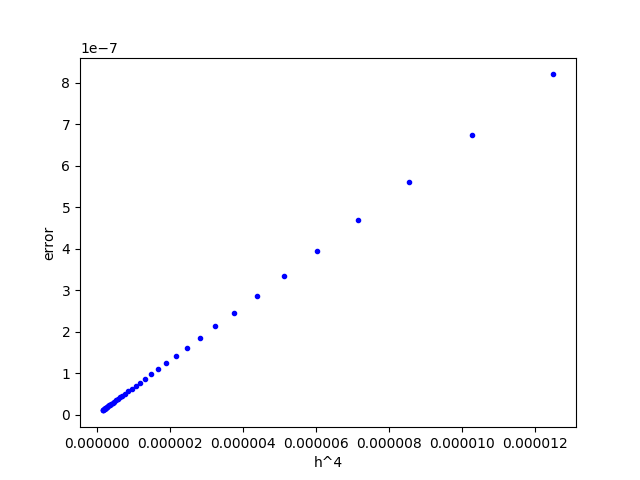
\includegraphics[width=.75\textwidth]{hw7_p1_fig2}
		\label{p1_T_corrected_err}
		\centering
	\end{figure}

\bigbreak
%%%%%%%%%%%%%%%%%%%%%%%%%%%%%%%%%%%%%%%%%%%%%%%%%%%%%%%%%%%%%%%%%%%%%%%%%%%%%%%%%%%%%%%%%%%%%%%%%%%%
\problem{1 (d)} The rate of the error of the Trapezoidal rule applied to $I(f_2)$ will acually decreace along $\mathcal{O}(h^4)$. This is because $f_2^\prime(-1)=0= f_2^\prime(1)$ and thus the correction term for the corrected Trapezoidal rule is $0$. For the same justification that the error of the corrected trapezoidal rule decreaces by $\mathcal{O}(h^4)$ we can justify that the uncorrected Trapazoidal rule will too, since it has the same value.

\bigbreak
%%%%%%%%%%%%%%%%%%%%%%%%%%%%%%%%%%%%%%%%%%%%%%%%%%%%%%%%%%%%%%%%%%%%%%%%%%%%%%%%%%%%%%%%%%%%%%%%%%%%
\problem{2 (a)} Construct the cubic Hermite interpolating polynomial $p(x)$ on the interval $[a,b]$ such that
\begin{align*}
	p(a) &= f(a) & p^\prime(a) &= f^\prime(a) \\
	p(b) &= f(b) & p^\prime(b) &= f^\prime(b)
\end{align*}

	We can use Newton's divided difference method to derive the cubic Hermite interpolating polynomial.
	\begin{center}
		\begin{tabular}{|c|c|c|c|c|}\hline
			$x_i$ & $f[\cdot]$ & $f[\cdot,\cdot]$ & $f[\cdot,\cdot,\cdot]$ & $f[\cdot,\cdot,\cdot,\cdot]$\\ \hline
			$a$ & $f(a)$ & & & \\ \hline
			$a$ & $f(a)$ & $f^\prime(a)$ & & \\ \hline
			$b$ & $f(b)$ & $f[a,b]$ & $\frac{f[a,b] - f^\prime(a)}{h}$ & \\ \hline
			$b$ & $f(b)$ & $f^\prime(b)$ & $\frac{f^\prime(b) - f[a,b]}{h}$ & $\frac{f^\prime(b) - 2f[a,b] + f^\prime(a)}{h^2}$ \\ \hline
		\end{tabular}
	\end{center}
	$$p(x) = f(a) + (x-a)f^\prime(a) + (x-a)^2 \frac{f[a,b]-f^\prime(a)}{h} + (x-b)(x-a)^2 \frac{f^\prime(b) - 2f[a,b] + f^\prime(a)}{h^2}$$

\bigbreak
%%%%%%%%%%%%%%%%%%%%%%%%%%%%%%%%%%%%%%%%%%%%%%%%%%%%%%%%%%%%%%%%%%%%%%%%%%%%%%%%%%%%%%%%%%%%%%%%%%%%
\problem{2 (b)} Using part (a), derive a cubic Hermite quadrature formula. \bigbreak

	If $p(x)$ is the cubic Hermite interpolating polynomial of $f(x)$ at the points $a$ and $b$ then the quadrature is given by
	\begin{align*}
		\int_a^b f(x) & \approx \int_a^b p(x) \\
		& = \int_a^b f(a) + (x-a)f^\prime(a) + (x-a)^2 \frac{f[a,b]-f^\prime(a)}{h} \\
		& \phantom{=====} + (x-b)(x-a)^2 \frac{f^\prime(b) - 2f[a,b] + f^\prime(a)}{h^2} dx \\
		& = hf(a) + \tfrac{1}{2}h^2f^\prime(a) + \tfrac{1}{3}h^2 (f[a,b]-f^\prime(a)) - \tfrac{1}{12}h^2 (f^\prime(b) - 2f[a,b] + f^\prime(a))
	\end{align*}
	
\bigbreak
%%%%%%%%%%%%%%%%%%%%%%%%%%%%%%%%%%%%%%%%%%%%%%%%%%%%%%%%%%%%%%%%%%%%%%%%%%%%%%%%%%%%%%%%%%%%%%%%%%%%
\problem{2 (c)} Give a formula for the error in part (a). \bigbreak 

	From class and the text we know that the error is given by
	$$
	\vert f(x) - p(x) \vert = \frac{(x-a)^2(x-b)^2}{4!}f^{(4)}(\xi)
	$$
	For some $\xi \in (a,b)$.
	
\bigbreak
%%%%%%%%%%%%%%%%%%%%%%%%%%%%%%%%%%%%%%%%%%%%%%%%%%%%%%%%%%%%%%%%%%%%%%%%%%%%%%%%%%%%%%%%%%%%%%%%%%%%
\problem{2 (d)} Derive the error for the quadrature formula in part (b). \bigbreak

	\begin{align*}
		\left \vert \int_a^b f(x) dx - \int_a^b p(x) dx \right \vert &= \left \vert \int_a^b f(x) - p(x) dx \right \vert \\
		& = \left \vert \int_a^b \frac{(x-a)^2(x-b)^2}{4!}f^{(4)}(\xi) dx \right \vert \\
		& = \left \vert \frac{h^5}{720}f^{(4)}(\xi) \right \vert \\
		& \leq \max_{x \in (a,b)}\left \vert \frac{h^5}{720}f^{(4)}(x) \right \vert
	\end{align*}
	
\bigbreak
%%%%%%%%%%%%%%%%%%%%%%%%%%%%%%%%%%%%%%%%%%%%%%%%%%%%%%%%%%%%%%%%%%%%%%%%%%%%%%%%%%%%%%%%%%%%%%%%%%%%
\problem{2 (e)} What is the degree of precision for the cubic Hermite quadrature formula? \bigbreak

	The degree of precision is 3, since the fourth derivative of cubic polynomials is always 0.
	
	
\bigbreak
%%%%%%%%%%%%%%%%%%%%%%%%%%%%%%%%%%%%%%%%%%%%%%%%%%%%%%%%%%%%%%%%%%%%%%%%%%%%%%%%%%%%%%%%%%%%%%%%%%%%
\problem{3 (a)} Using the 5-node GQ formula in the provided Mathematica script, the nodes and weights for the integral $\int_0^1 f(x)\log(\tfrac{1}{x})dx$ have been calculated as follows\\
\begin{center}
	\begin{tabular}{|c|c|c|}\hline
		$i$ & $x_i$ & $w_i$\\ \hline
		0 & 0.029134472151 & 0.2978934717828945 \\ \hline
		1 & 0.173977213320 & 0.3497762265132242 \\ \hline
		2 & 0.411702520284 & 0.2344882900440524 \\ \hline
		3 & 0.677314174582 & 0.09893045951663315 \\ \hline
		4 & 0.894771361031 & 0.01891155214319580 \\ \hline
	\end{tabular}
\end{center}

\bigbreak
%%%%%%%%%%%%%%%%%%%%%%%%%%%%%%%%%%%%%%%%%%%%%%%%%%%%%%%%%%%%%%%%%%%%%%%%%%%%%%%%%%%%%%%%%%%%%%%%%%%%
\problem{3 (b)} The code below uses the nodes and weights calculated above to determine $\int_0^1 \sin(x)\log(\tfrac{1}{x})dx \approx 0.239811742000565$. The output shows that the error is $7.71049890602\times 10^{-14}$. This is a very good approximation for using only samplings of the function.

\begin{lstlisting}
def p3b():
	xs = [0.02913447215197205,
		0.1739772133208976,
		0.4117025202849020,
		0.6773141745828204,
		0.8947713610310083]
	ws = [0.2978934717828945,
		0.3497762265132242,
		0.2344882900440524,
		0.09893045951663315,
		0.01891155214319580]
	correct = 0.239811742000565
	ys = np.sin(xs)
	GQ = np.dot(ws,ys)
	print("Gaussian Quadrature:")
	print(GQ)
	print("Error: ")
	print((GQ - correct))

**********************************
Output:
>>> p3b()
Gaussian Quadrature:
0.239811742001
Error: 
7.71049890602e-14
\end{lstlisting}

\bigbreak
%%%%%%%%%%%%%%%%%%%%%%%%%%%%%%%%%%%%%%%%%%%%%%%%%%%%%%%%%%%%%%%%%%%%%%%%%%%%%%%%%%%%%%%%%%%%%%%%%%%%
\problem{3 (c)} The nodes and weights for GQ applied to the function $\int_0^1 f(x)dx$ are below. After is a program using these weights to calculate the same integral as above. The error can be seen to be far less acurate: error$= 0.000285041178903$. Knowing the weight function in advance greatly improves the GQ algorithm.
\begin{center}
	\begin{tabular}{|c|c|c|}\hline
		$i$ & $x_i$ & $w_i$\\ \hline
		0 & 0.04691007703066800 & 0.1184634425280945 \\ \hline
		1 & 0.2307653449471585 & 0.2393143352496832 \\ \hline
		2 & 0.5 & 0.2844444444444444 \\ \hline
		3 & 0.7692346550528415 & 0.2393143352496832 \\ \hline
		4 & 0.9530899229693320 & 0.1184634425280945 \\ \hline	
	\end{tabular}
\end{center}
\begin{lstlisting}
def p3c():
	xs = [0.04691007703066800,
		0.2307653449471585,
		0.5000000000000000,
		0.7692346550528415,
		0.9530899229693320]
	ws = [0.1184634425280945,
		0.2393143352496832,
		0.2844444444444444,
		0.2393143352496832,
		0.1184634425280945]
	correct = 0.239811742000565
	ys = np.sin(xs)*np.log(1.0/np.array(xs))
	GQ = np.dot(ws,ys)
	print("Gaussian Quadrature:")
	print(GQ)
	print("Error: ")
	print((GQ - correct))

**********************************
Output:
>>> p3c()
Gaussian Quadrature:
0.240096783179
Error: 
0.000285041178903
\end{lstlisting}

\bigbreak
%%%%%%%%%%%%%%%%%%%%%%%%%%%%%%%%%%%%%%%%%%%%%%%%%%%%%%%%%%%%%%%%%%%%%%%%%%%%%%%%%%%%%%%%%%%%%%%%%%%%
\problem{3 (d)} Using 11 node GQ on $\int_0^1 f(x) dx$ we obtain the nodes and weights below. Usint them to evaluate the same integral as above the program below gives us the error: $1.44841479686\times 10^{-5}$. Knowing the weight function in advance is marvelous indeed!
\begin{center}
	\begin{tabular}{|c|c|c|}
		\hline
		$i$&$x_i$&$w_i$\\ \hline
		0&0.0108856709269715&0.02783428355808683\\ \hline
		1&0.05646870011595235&0.0627901847324523\\ \hline
		2&0.1349239972129753&0.09314510546386713\\ \hline
		3&0.2404519353965941&0.1165968822959952\\ \hline
		4&0.3652284220238275&0.1314022722551233\\ \hline
		5&0.5&0.1364625433889503\\ \hline
		6&0.6347715779761725&0.1314022722551233\\ \hline
		7&0.7595480646034058&0.1165968822959952\\ \hline
		8&0.8650760027870247&0.09314510546386713\\ \hline
		9&0.9435312998840476&0.0627901847324523\\ \hline
		10&0.9891143290730285&0.02783428355808683\\ \hline
	\end{tabular}
\end{center}
\begin{lstlisting}
def p3d():
	xs = [0.01088567092697150,
		0.05646870011595235,
		0.1349239972129753,
		0.2404519353965941,
		0.3652284220238275,
		0.5,
		0.6347715779761725,
		0.7595480646034059,
		0.8650760027870247,
		0.9435312998840476,
		0.9891143290730285]
	ws = [0.02783428355808683,
		0.06279018473245231,
		0.09314510546386713,
		0.1165968822959952,
		0.1314022722551233,
		0.1364625433889503,
		0.1314022722551233,
		0.1165968822959952,
		0.09314510546386713,
		0.06279018473245231,
		0.02783428355808683]
correct = 0.239811742000565
ys = np.sin(xs)*np.log(1.0/np.array(xs))
GQ = np.dot(ws,ys)
print("Gaussian Quadrature:")
print(GQ)
print("Error: %f")
print((GQ - correct))

**********************************
Output:
>>> p3d()
Gaussian Quadrature:
0.239826226149
Error: %f
1.44841479686e-05
\end{lstlisting}

\bigbreak
%%%%%%%%%%%%%%%%%%%%%%%%%%%%%%%%%%%%%%%%%%%%%%%%%%%%%%%%%%%%%%%%%%%%%%%%%%%%%%%%%%%%%%%%%%%%%%%%%%%%
\problem{4 (a)}

\bigbreak
%%%%%%%%%%%%%%%%%%%%%%%%%%%%%%%%%%%%%%%%%%%%%%%%%%%%%%%%%%%%%%%%%%%%%%%%%%%%%%%%%%%%%%%%%%%%%%%%%%%%
\problem{4 (b)}

\begin{center}
	\begin{tabular}{|c|c|c|}
		\hline
		$n$&$R_{i,i}$&err\\ \hline
		1&3.0&-0.14159265359\\ \hline
		2&3.13333333333&-0.00825932025646\\ \hline
		4&3.14211764706&0.000524993469031\\ \hline
		8&3.14158578376&-6.86982791853e-06\\ \hline
		16&3.14159266528&1.1687923962e-08\\ \hline
		32&3.14159265364&4.84510209731e-11\\ \hline
	\end{tabular}
\end{center}

	
\bigbreak
%%%%%%%%%%%%%%%%%%%%%%%%%%%%%%%%%%%%%%%%%%%%%%%%%%%%%%%%%%%%%%%%%%%%%%%%%%%%%%%%%%%%%%%%%%%%%%%%%%%%
\problem{6 (a)} See that
\begin{align*}
	1 + \sum_{k=2}^\infty \Big [ \tfrac{1}{k} + \log(1-\tfrac{1}{k}) \Big] & = 1 + \lim_{N \to \infty} \sum_{k=2}^N \Big [ \tfrac{1}{k} + \log(1-\tfrac{1}{k}) \Big] \\
	& = 1 + \lim_{n \to \infty} \sum_{k=2}^n \tfrac{1}{k} + \sum_{k=2}^n \log(1-\tfrac{1}{k}) \\
	& = \lim_{n \to \infty} \sum_{k=1}^n \tfrac{1}{k} + \sum_{k=2}^n \log(1-\tfrac{1}{k}) \\
	& = \lim_{n \to \infty} \left( \sum_{k=1}^n \tfrac{1}{k} \right) + \log \left( \prod_{k=2}^n 1-\tfrac{1}{k} \right) \\
	& = \lim_{n \to \infty} \left( \sum_{k=1}^n \tfrac{1}{k} \right) + \log \left( \prod_{k=2}^n \tfrac{k-1}{k} \right) \\
	& = \lim_{n \to \infty} \left( \sum_{k=1}^n \tfrac{1}{k} \right) + \log \left( \frac{(n-1)!}{n!} \right) \\
	& = \lim_{n \to \infty} \left( \sum_{k=1}^n \tfrac{1}{k} \right) + \log \left( n^{-1} \right) \\
	& = \lim_{n \to \infty} \left( \sum_{k=1}^n \tfrac{1}{k} \right) - \log \left( n \right) \\
	& = \gamma = 0.5772156649015328\dots
\end{align*}

\bigbreak
%%%%%%%%%%%%%%%%%%%%%%%%%%%%%%%%%%%%%%%%%%%%%%%%%%%%%%%%%%%%%%%%%%%%%%%%%%%%%%%%%%%%%%%%%%%%%%%%%%%%
\problem{6 (b)} Using the Euler-MacLaurin formula after suming the first $k=2, \dots,20$ terms we can approximate $\gamma$. Let $f(x) = \frac{1}{x} + \log(1-\tfrac{1}{x})$. Then we use the following facts to do so
\begin{align*}
	\int_20^\infty f(x) dx & = 38\tanh^{-1}(\tfrac{1}{39}) -1 \\
	f^\prime(x) & = -x^{-2} - x^{-1} + (x-1)^{-1} \\
	f^{\prime\prime\prime}(x) & = -6x^{-4} - 2x^{-3} + 2(x-1)^{-3} \\
	f^{(5)}(x) & = -120x^{-6} - 24x^{-5} + 24(x-1)^{-5}
\end{align*}
This is done in the following program
\begin{lstlisting}
gamma = 0.5772156649015328

def p6_f(x):
	return 1/x + np.log(1-1/x)
	
def p6_f1(x):
	return -x**-2 + (x-1)**-1 - x**-1
	
def p6_f3(x):
	return -6*x**-4 + 2*(x-1)**-3 - 2*x**-3
	
def p6_f5(x):
	return -120*x**-6 + 24*(x-1)**-5 - 24*x**-5
	
def euler_maclaurin_terms(N):
	return p6_f(N)/2 - p6_f1(N)/12 + p6_f3(N)/720 - p6_f5(N)/30240

def gamma_approx():
	gamma_approx = 1
	for k in range(2,20):
		gamma_approx += 1/k + np.log(1-1/k)
		gamma_approx += 38*np.arctanh(1/39)-1 + euler_maclaurin_terms(20)
	return gamma_approx
\end{lstlisting}

When executed it approximates $\gamma \approx 0.577215664901$ for which the error is $3.74145159299 \times 10^{-14}$

\bigbreak
%%%%%%%%%%%%%%%%%%%%%%%%%%%%%%%%%%%%%%%%%%%%%%%%%%%%%%%%%%%%%%%%%%%%%%%%%%%%%%%%%%%%%%%%%%%%%%%%%%%%
\problem{6 (c)} When summed directly the first 1000 terms of the series give an error of $0.000498918995019$. This is far worse than using the Euler MacLaurin formula. This calculation is performed in the following program.

\begin{lstlisting}
def p6c():
	approx = 1
	for k in range(2,1003):
		approx += 1/k + np.log(1-1/k)
	print(approx - gamma)
\end{lstlisting}



\end{document}
